% questions.tex —— 2013 年·重庆卷·文科 · 题目内容片段（无答案）
% 由 tools/generate_projects.py 依来源总账自 2013/2013_数学真题_重庆文_试题.md 生成，勿手改（改源 MD 后重跑）
\gkpart{一、选择题}
\begin{question}
\gkti{1}已知全集 $U=\{1,2,3,4\}$，集合 $A=\{1,2\}$，$B=\{2,3\}$，则 $\complement_U(A\cup B)=$\mbox{（　　）}
（A）$\{1,3,4\}$；（B）$\{3,4\}$；（C）$\{3\}$；（D）$\{4\}$。
\end{question}
\begin{question}
\gkti{2}命题“对任意 $x\in\mathbf R$，都有 $x^2\geqslant0$”的否定为\mbox{（　　）}
（A）存在 $x_0\in\mathbf R$，使得 $x_0^2<0$；（B）不存在 $x\in\mathbf R$，使得 $x^2<0$；（C）存在 $x_0\in\mathbf R$，使得 $x_0^2\geqslant0$；（D）对任意 $x\in\mathbf R$，都有 $x^2<0$。
\end{question}
\begin{question}
\gkti{3}函数 $y=\dfrac1{\log_2(x-2)}$ 的定义域是\mbox{（　　）}
（A）$(-\infty,2)$；（B）$(2,+\infty)$；（C）$(2,3)\cup(3,+\infty)$；（D）$(2,4)\cup(4,+\infty)$。
\end{question}
\begin{question}
\gkti{4}设 $P$ 是圆 $(x-3)^2+(y+1)^2=4$ 上的动点，$Q$ 是直线 $x=-3$ 上的动点，则 $|PQ|$ 的最小值为\mbox{（　　）}
（A）$6$；（B）$4$；（C）$3$；（D）$2$。
\Needspace{0.4\textheight}
\end{question}
\begin{question}
\gkti{5}执行如图所示的程序框图，则输出的 $k$ 的值是\mbox{（　　）}
\nopagebreak[4]
\begin{center}% 2013 重庆卷文科第 5 题：输出 k 的值的程序框图。
\begin{tikzpicture}[font=\footnotesize, >=Stealth, line width=0.45pt,
  node distance=4.8mm,
  term/.style={draw, rounded corners=5pt, minimum height=1.8em, inner xsep=8pt},
  io/.style={draw, trapezium, trapezium left angle=72, trapezium right angle=108,
             minimum height=1.8em, inner xsep=7pt},
  box/.style={draw, minimum height=1.8em, inner xsep=6pt},
  dec/.style={draw, diamond, aspect=2.6, inner sep=1pt}]
  \node[term] (start) {开始};
  \node[box, below=5mm of start] (init) {$k=1$，$s=1$};
  \node[box, below=8mm of init] (acc) {$s=s+(k-1)^2$};
  \node[dec, below=6mm of acc] (test) {$s>15$?};
  \node[box, right=11mm of test] (inc) {$k=k+1$};
  \node[io, below=10mm of test] (output) {输出 $k$};
  \node[term, below=5mm of output] (end) {结束};
  \draw[->] (start) -- (init);
  \draw[->] (init) -- (acc);
  \draw[->] (acc) -- (test);
  \draw[->] (test) -- node[right] {是} (output);
  \draw[->] (test) -- node[above] {否} (inc);
  \draw[->] (output) -- (end);
  % 否分支回到累加框上方
  \coordinate (loop) at ($(acc.north)+(0.55,0.40)$);
  \coordinate (loopt) at ($(acc.north)+(0.55,0)$);
  \draw[->] (inc.north) -- (inc.north |- loop) -- (loop) -- (loopt);
\end{tikzpicture}
\end{center}
\nopagebreak[4]
（A）$3$；（B）$4$；（C）$5$；（D）$6$。
\Needspace{0.4\textheight}
\end{question}
\begin{question}
\gkti{6}如图是某公司 $10$ 个销售店某月销售某产品数量（单位：台）的茎叶图，则数据落在区间 $[22,30)$ 内的频率为\mbox{（　　）}
\nopagebreak[4]
\begin{center}% 2013 重庆卷文科第 6 题：10 个销售店某月销售某产品数量的茎叶图。
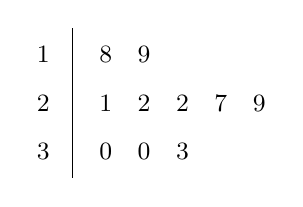
\begin{tikzpicture}[font=\small, line width=0.45pt]
  % 茎（十位）
  \node[anchor=east] at (0,0.62) {1};
  \node[anchor=east] at (0,0) {2};
  \node[anchor=east] at (0,-0.62) {3};
  % 分隔竖线
  \draw (0.16,0.95) -- (0.16,-0.95);
  % 叶（个位）
  \node[anchor=west] at (0.38,0.62) {8\quad 9};
  \node[anchor=west] at (0.38,0) {1\quad 2\quad 2\quad 7\quad 9};
  \node[anchor=west] at (0.38,-0.62) {0\quad 0\quad 3};
\end{tikzpicture}
\end{center}
\nopagebreak[4]
（A）$0.2$；（B）$0.4$；（C）$0.5$；（D）$0.6$。
\end{question}
\begin{question}
\gkti{7}关于 $x$ 的不等式 $x^2-2ax-8a^2<0$（$a>0$）的解集为 $(x_1,x_2)$，且 $x_2-x_1=15$，则 $a=$\mbox{（　　）}
（A）$\dfrac52$；（B）$\dfrac72$；（C）$\dfrac{15}4$；（D）$\dfrac{15}2$。
\Needspace{0.4\textheight}
\end{question}
\begin{question}
\gkti{8}某几何体的三视图如图所示，则该几何体的表面积为\mbox{（　　）}
\nopagebreak[4]
\begin{center}% 2013 重庆卷文科第 8 题：几何体的三视图。
% 正（主）视图为 10×4 的矩形；侧（左）视图为下底 8、上底 2、高 4 的等腰梯形；
% 俯视图为 10×8 的矩形，被两条与长边平行的线分成 3、2、3 三部分。
\begin{tikzpicture}[font=\small, >=Stealth, line width=0.45pt, x=0.26cm, y=0.26cm]
  % ---- 正（主）视图：10 宽、4 高 ----
  \draw (0,0) rectangle (10,4);
  % 尺寸 4
  \draw[<->] (-2,0) -- (-2,4);
  \draw (-2.8,0) -- (-1.2,0);
  \draw (-2.8,4) -- (-1.2,4);
  \node[left] at (-2.8,2) {4};
  % 尺寸 10
  \draw[<->] (0,-2) -- (10,-2);
  \draw (0,-2.8) -- (0,-1.2);
  \draw (10,-2.8) -- (10,-1.2);
  \node[below] at (5,-2.2) {10};
  \node[below] at (5,-3.6) {正（主）视图};

  % ---- 侧（左）视图：下底 8、上底 2、高 4 的等腰梯形 ----
  \begin{scope}[shift={(13.8,0)}]
    \draw (0,0) -- (8,0) -- (5,4) -- (3,4) -- cycle;
    \draw[<->] (0,-2) -- (8,-2);
    \draw (0,-2.8) -- (0,-1.2);
    \draw (8,-2.8) -- (8,-1.2);
    \node[below] at (4,-2.2) {8};
    \node[below] at (4,-3.6) {侧（左）视图};
  \end{scope}

  % ---- 俯视图：10×8 的矩形，分成 3、2、3 ----
  \begin{scope}[shift={(0,-14)}]
    \draw (0,0) rectangle (10,8);
    \draw (0,5.7) -- (10,5.7);
    \draw (0,3.3) -- (10,3.3);
    % 左侧尺寸 3、2、3
    \draw[<->] (-2,5.7) -- (-2,8);
    \draw[<->] (-2,3.3) -- (-2,5.7);
    \draw[<->] (-2,0) -- (-2,3.3);
    \draw (-2.8,0) -- (-1.2,0);
    \draw (-2.8,3.3) -- (-1.2,3.3);
    \draw (-2.8,5.7) -- (-1.2,5.7);
    \draw (-2.8,8) -- (-1.2,8);
    \node[left] at (-2.8,6.85) {3};
    \node[left] at (-2.8,4.5) {2};
    \node[left] at (-2.8,1.65) {3};
    \node[below] at (5,-1.4) {俯视图};
  \end{scope}
\end{tikzpicture}
\end{center}
\nopagebreak[4]
（A）$180$；（B）$200$；（C）$220$；（D）$240$。
\end{question}
\begin{question}
\gkti{9}已知函数 $f(x)=ax^3+b\sin x+4$（$a,b\in\mathbf R$），$f(\lg(\log_2 10))=5$，则 $f(\lg(\lg 2))=$\mbox{（　　）}
（A）$-5$；（B）$-1$；（C）$3$；（D）$4$。
\end{question}
\begin{question}
\gkti{10}设双曲线 $C$ 的中心为点 $O$，若有且只有一对相交于点 $O$、所成的角为 $60^\circ$ 的直线 $A_1B_1$ 和 $A_2B_2$，使 $|A_1B_1|=|A_2B_2|$，其中 $A_1$，$B_1$ 和 $A_2$，$B_2$ 分别是这对直线与双曲线 $C$ 的交点，则该双曲线的离心率的取值范围是\mbox{（　　）}
（A）$\left(\dfrac{2\sqrt3}3,2\right]$；（B）$\left[\dfrac{2\sqrt3}3,2\right)$；（C）$\left(\dfrac{2\sqrt3}3,+\infty\right)$；（D）$\left[\dfrac{2\sqrt3}3,+\infty\right)$。
\end{question}
\gkpart{二、填空题}
\begin{question}
\gkti{11}设复数 $z=1+2\mathrm i$（$\mathrm i$ 是虚数单位），则 $|z|=$\gkblank{}。
\end{question}
\begin{question}
\gkti{12}若 $2$，$a$，$b$，$c$，$9$ 成等差数列，则 $c-a=$\gkblank{}。
\end{question}
\begin{question}
\gkti{13}若甲、乙、丙三人随机地站成一排，则甲、乙两人相邻而站的概率为\gkblank{}。
\end{question}
\begin{question}
\gkti{14}在 $\overrightarrow{OA}$ 为边、$\overrightarrow{OB}$ 为对角线的矩形中，已知 $\overrightarrow{OA}=(-3,1)$，$\overrightarrow{OB}=(-2,k)$，则实数 $k=$\gkblank{}。
\end{question}
\begin{question}
\gkti{15}设 $0\leqslant\alpha\leqslant\pi$，不等式 $8x^2-(8\sin\alpha)x+\cos2\alpha\geqslant0$ 对 $x\in\mathbf R$ 恒成立，则 $\alpha$ 的取值范围为\gkblank{}。
\end{question}
\gkpart{三、解答题}
\begin{question}
\gkti{16}设数列 $\{a_n\}$ 满足：$a_1=1$，$a_{n+1}=3a_n$，$n\in\mathbf N_+$。
（1） 求 $\{a_n\}$ 的通项公式及前 $n$ 项和 $S_n$；
（2） 已知 $\{b_n\}$ 是等差数列，$T_n$ 为其前 $n$ 项和，且 $b_1=a_2$，$b_3=a_1+a_2+a_3$，求 $T_{20}$。
\end{question}
\begin{question}
\gkti{17}从某居民区随机抽取 $10$ 个家庭，获得第 $i$ 个家庭的月收入 $x_i$（单位：千元）与月储蓄 $y_i$（单位：千元）的数据资料，算得 $\sum\limits_{i=1}^{10}x_i=80$，$\sum\limits_{i=1}^{10}y_i=20$，$\sum\limits_{i=1}^{10}x_iy_i=184$，$\sum\limits_{i=1}^{10}x_i^2=720$。
（1） 求家庭的月储蓄 $y$ 对月收入 $x$ 的线性回归方程 $\hat y=\hat bx+\hat a$；
（2） 判断变量 $x$ 与 $y$ 之间是正相关还是负相关；
（3） 若该居民区某家庭月收入为 $7$ 千元，预测该家庭的月储蓄。
附：线性回归方程 $\hat y=\hat bx+\hat a$ 中，$\hat b=\dfrac{\sum\limits_{i=1}^n x_iy_i-n\bar x\bar y}{\sum\limits_{i=1}^n x_i^2-n\bar x^2}$，$\hat a=\bar y-\hat b\bar x$，其中 $\bar x$，$\bar y$ 为样本平均值，线性回归方程也可写为 $\hat y=\hat bx+\hat a$。
\end{question}
\begin{question}
\gkti{18}在 $\triangle ABC$ 中，内角 $A$，$B$，$C$ 的对边分别为 $a$，$b$，$c$，且 $a^2=b^2+c^2+\sqrt3bc$。
（1） 求 $A$；
（2） 设 $a=\sqrt3$，$S$ 为 $\triangle ABC$ 的面积，求 $S+\sqrt3\cos B\cos C$ 的最大值，并指出此时 $B$ 的值。
\Needspace{0.4\textheight}
\end{question}
\begin{question}
\gkti{19}如图，四棱锥 $P-ABCD$ 中，$PA\perp$ 底面 $ABCD$，$PA=2\sqrt3$，$BC=CD=2$，$\angle ACB=\angle ACD=\dfrac\pi3$。
\nopagebreak[4]
\begin{center}% 2013 重庆卷文科第 19 题：四棱锥 P-ABCD，PA 垂直于底面，
% F 在棱 PC 上且 PF=7FC。
\begin{tikzpicture}[font=\small, line width=0.45pt, scale=1]
  \coordinate (P) at (-0.15,3.40);
  \coordinate (A) at (0,0);
  \coordinate (B) at (1.60,-1.50);
  \coordinate (C) at (4.10,-0.70);
  \coordinate (D) at (3.20,1.40);
  \coordinate (F) at ($(P)!0.875!(C)$);
  % 可见棱
  \draw (P) -- (A);
  \draw (P) -- (B);
  \draw (P) -- (C);
  \draw (P) -- (D);
  \draw (A) -- (B);
  \draw (B) -- (C);
  \draw (C) -- (D);
  \draw (D) -- (A);
  % 不可见棱
  \draw[dashed] (A) -- (C);
  \draw[dashed] (B) -- (D);
  \draw[dashed] (B) -- (F);
  % 顶点标注
  \node[above left] at (P) {$P$};
  \node[below left] at (A) {$A$};
  \node[below] at (B) {$B$};
  \node[right] at (C) {$C$};
  \node[above right] at (D) {$D$};
  \node[left] at (F) {$F$};
\end{tikzpicture}
\end{center}
\nopagebreak[4]
（1） 求证：$BD\perp$ 平面 $PAC$；
（2） 若侧棱 $PC$ 上的点 $F$ 满足 $PF=7FC$，求三棱锥 $P-BDF$ 的体积。
\end{question}
\begin{question}
\gkti{20}某村庄拟修建一个无盖的圆柱形蓄水池（不计厚度）。设该蓄水池的底面半径为 $r$ 米，高为 $h$ 米，体积为 $V$ 立方米。假设建造成本仅与表面积有关，侧面的建造成本为 $100$ 元/平方米，底面的建造成本为 $160$ 元/平方米，该蓄水池的总建造成本为 $12000\pi$ 元（$\pi$ 为圆周率）。
（1） 将 $V$ 表示成 $r$ 的函数 $V(r)$，并求该函数的定义域；
（2） 讨论函数 $V(r)$ 的单调性，并确定 $r$ 和 $h$ 为何值时该蓄水池的体积最大。
\Needspace{0.4\textheight}
\end{question}
\begin{question}
\gkti{21}如图，椭圆的中心为原点 $O$，长轴在 $x$ 轴上，离心率 $e=\dfrac{\sqrt2}2$，过左焦点 $F_1$ 作 $x$ 轴的垂线交椭圆于 $A$，$A'$ 两点，$|AA'|=4$。
\nopagebreak[4]
\begin{center}% 2013 重庆卷文科第 21 题：椭圆与内切圆 Q。
% 椭圆 x^2/16+y^2/8=1，图中按 1:2 缩小绘制（半长轴 2，半短轴 sqrt2）。
\begin{tikzpicture}[font=\small, line width=0.45pt, >=Stealth, scale=1]
  \def\aa{2}
  \def\bb{1.41421}
  \def\cc{1.41421}
  \def\yy{1}
  % 椭圆
  \draw (0,0) ellipse ({\aa} and {\bb});
  % 坐标轴
  \draw[->] (-2.85,0) -- (2.95,0) node[below] {$x$};
  \draw[->] (0,-1.95) -- (0,2.05) node[right] {$y$};
  \node[below left] at (0,0) {$O$};
  % 过左焦点 F1 的垂线，交椭圆于 A、A'
  \draw (-\cc,-1.16) -- (-\cc,1.16);
  \fill (-\cc,0) circle (0.6pt);
  \node[below right] at (-\cc,0) {$F_1$};
  \node[above left] at (-\cc,\yy) {$A$};
  \node[below left] at (-\cc,-\yy) {$A'$};
  % 过 P、P' 的弦
  \draw (\cc,-1.16) -- (\cc,1.16);
  \node[above left] at (\cc,\yy) {$P$};
  \node[below left] at (\cc,-\yy) {$P'$};
  % 圆 Q：圆心 (sqrt2/2,0)，半径 sqrt6/2
  \draw (0.70711,0) circle (1.22474);
  \fill (0.70711,0) circle (0.9pt);
  \node[below left] at (0.70711,0) {$Q$};
  % 半径 QP、QP'
  \draw (0.70711,0) -- (\cc,\yy);
  \draw (0.70711,0) -- (\cc,-\yy);
\end{tikzpicture}
\end{center}
\nopagebreak[4]
（1） 求该椭圆的标准方程；
（2） 取平行于 $y$ 轴的直线与椭圆相交于不同的两点 $P$，$P'$，过 $P$，$P'$ 作圆心为 $Q$ 的圆，使椭圆上的其余点均在圆 $Q$ 外。求 $\triangle PP'Q$ 的面积 $S$ 的最大值，并写出对应的圆 $Q$ 的标准方程。

\end{question}